\chapter{Wygląd aplikacji}
Dodatek ten zawiera zrzuty ekranu przedstawiające wygląd zrealizowanej aplikacji.

\begin{figure}[]
    \begin{center}
	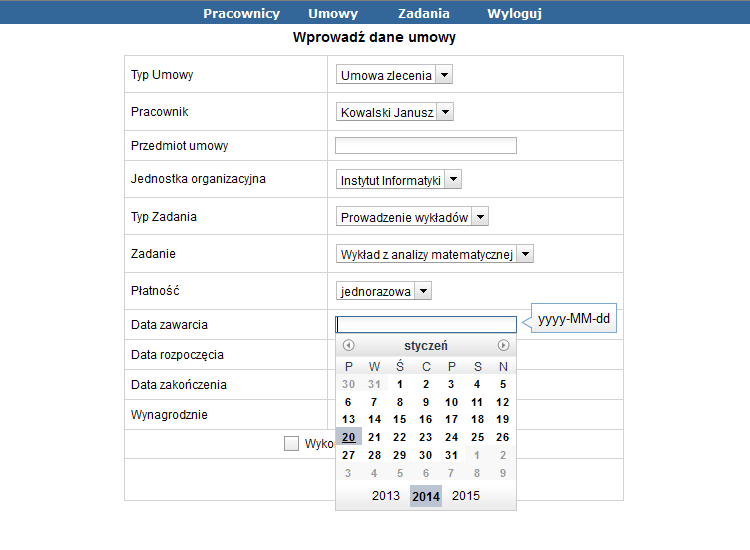
\includegraphics[scale=1,angle=-90]{img/screen1.png}
	\caption{Formularz służący do wprowadzania umowy}
	\label{screen1}
    \end{center}
\end{figure}

\begin{figure}[]
    \begin{center}
	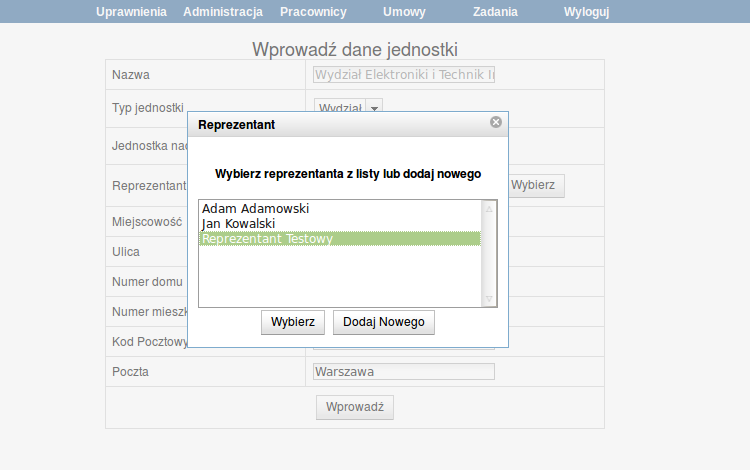
\includegraphics[scale=1,angle=-90]{img/screen2.png}
	\caption{Okno dialogowe pozwaljące na wybór Urzędu Skarbowego}
	\label{screen2}
    \end{center}
\end{figure}

\begin{figure}[]
    \begin{center}
	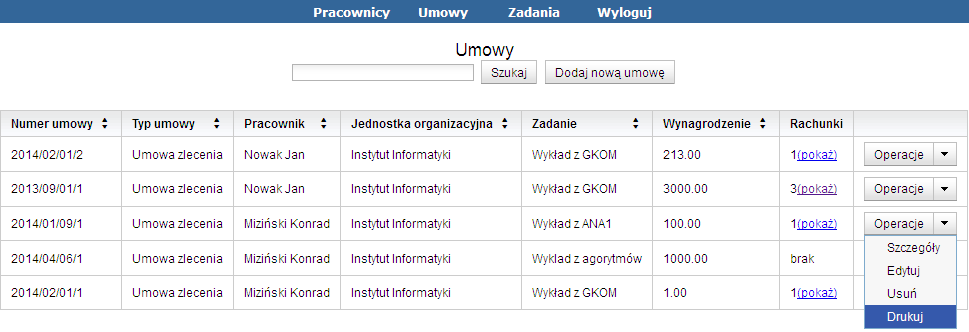
\includegraphics[scale=.8,angle=-90]{img/screen3.png}
	\caption{Sortowalna tabela z umowami}
	\label{screen3}
    \end{center}
\end{figure}

\begin{figure}[]
    \begin{center}
	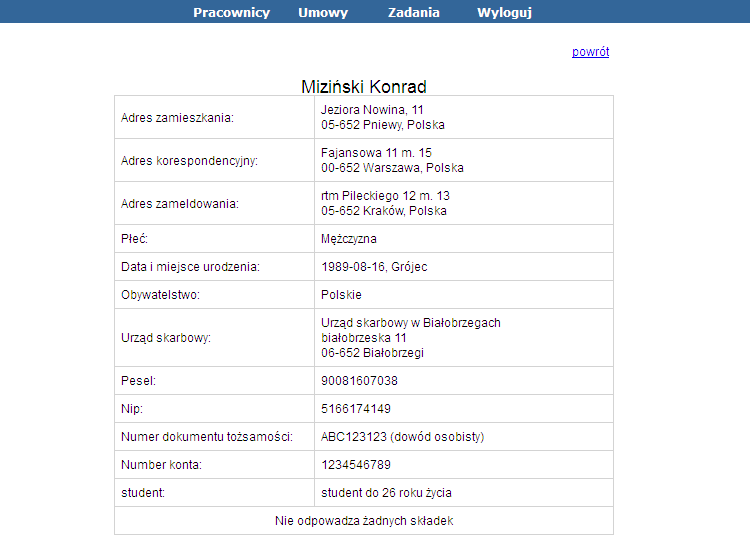
\includegraphics[scale=1,angle=-90]{img/screen4.png}
	\caption{Podsumowanie danych pracownika}
	\label{screen4}
    \end{center}
\end{figure}

\begin{figure}[]
    \begin{center}
	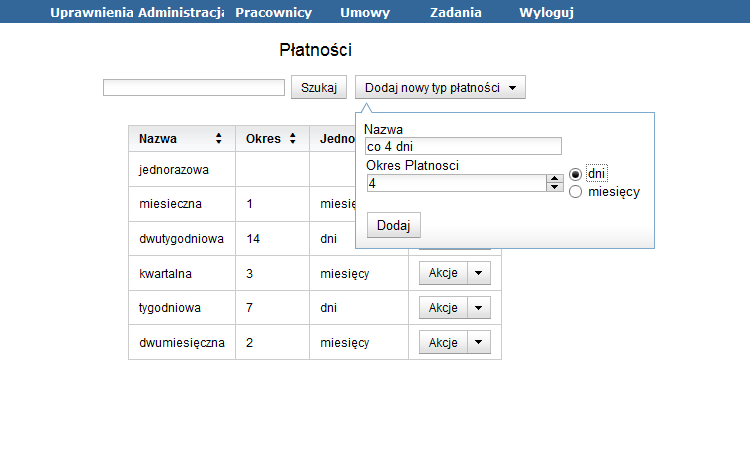
\includegraphics[scale=1,angle=-90]{img/screen5.png}
	\caption{Formularz w formie tooltipu do wpradzania płatności}
	\label{screen5}
    \end{center}
\end{figure}
